\section{Formale Sprachen}

Formale Sprache\footnote{\url{https://de.wikipedia.org/wiki/Formale\_Sprache}}
L über Alphabet $\Sigma$\\
L $\subseteq$ $\Sigma$*\\
% @todo: URL kleensche Hülle korrigieren
mit $\Sigma$* = Kleensche Hülle\footnote{\url{https://de.wikipedia.org/wiki/Kleenesche\_und\_positive\_H\%C3\%BClle}} von $\Sigma$\\


$$\Sigma^* = \bigcup_{n=0}^{\infty} \Sigma^{n}$$\\
$\Sigma^0 = \{\varepsilon\}, \Sigma^1 = \Sigma, \Sigma^2 = \Sigma \times \Sigma$\\
$\varepsilon \to$ leeres Wort (leere Menge)\\

Beispiel: $\Sigma = \{a\}, \Sigma^*=\{\varepsilon, a, aa, aaa, ...\}, L = \{a, aa, aaaa, ...\}$

\subsection{formale Grammatik G}

G = (N, $\Sigma$, P, S) mit\\
\begin{itemize}
	\item N = Nichtterminale
	\item $\Sigma$ = Alphabet
	\item P = Produktionsregeln
	\item S = Startsymbol ($\epsilon$ N)
\end{itemize}

% @todo: was bedeutet diese Zeile?
P $\subseteq (N \cup \Sigma)^* / N(N \cup \Sigma)^* \to (N \cup \Sigma)^*$\\
\\
Beispiel:\\
% @todo: die Produktionsregeln von links nach rechts anwenden wenn es mehrere gibt?
G=(\{S\}, \{a\}, $\{S \to aaS, S \to a\}$, S)\\
führt zu: S $\to$ aaS $\to$ aaa

\subsection{Klassifikation von formalen Sprachen}
durch die Comsky-Hierarchie\footnote{\url{https://de.wikipedia.org/wiki/Chomsky-Hierarchie}}:
\begin{itemize}
	\item Typ 0 = rekursiv auszählbar ($\alpha N \beta \to \gamma$)
	\item Typ 1 = kontext-sensitiv ($\alpha N \beta \to \alpha \gamma \beta$)
	\item Typ 2 = kontext-frei, N $\to (N \cup \Sigma)^* \to$ stochstisch kontextfreie Grammatik (SCFG) $\to$ Dynamics Programming
	\item Typ 3 = regular ($N \to \Sigma | \Sigma N$) $\to$ dann immer Hidden Markov Model (HMM) modellierbar
\end{itemize}

bei Alignments:
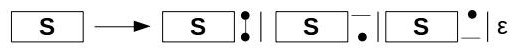
\includegraphics[width=0.7\textwidth]{lectures/160523_2/pix/1.jpg}
\\\\
Erweiterung mit Wahrscheinlichkeit:
G=(N, $\Sigma$, P, S, $\Omega$)\\
mit $\Omega$ = Wahrscheinlichkeit für Produktionsregeln\\
\\

\underline{jetzt auf RNA-Vorhersagen:}\\
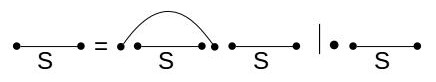
\includegraphics[width=0.7\textwidth]{lectures/160523_2/pix/2.jpg}

scoring scheme: Bewertung von 
$\sigma$ (
\includegraphics[width=0.05\textwidth]{lectures/160523_2/pix/4.jpg}) = 1, 
($\sigma$ (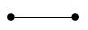
\includegraphics[width=0.05\textwidth]{lectures/160523_2/pix/3.jpg})), 
$\sigma$ (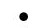
\includegraphics[width=0.05\textwidth]{lectures/160523_2/pix/5.jpg}) = 0\\
scoring function:
\begin{itemize}
	\item max Basepairs: + (Summe),
	\item Anzahl der Strukturen: $\cdot$ (Multiplikation)
\end{itemize}
choice function:
\begin{itemize}
	\item max Basepairs: max,
	\item Anzahl der Strukturen: + (Summe)
\end{itemize}

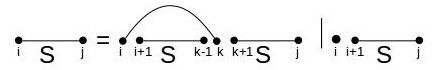
\includegraphics[width=0.7\textwidth]{lectures/160523_2/pix/6.jpg}
\\\\
$S_{ij}=\begin{cases}
               S_{i+1, j} + \sigma((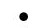
\includegraphics[width=0.05\textwidth]{lectures/160523_2/pix/5.jpg})\\
               S_{i+1, k-1} + S_{k+1,j} + \sigma((
\includegraphics[width=0.05\textwidth]{lectures/160523_2/pix/4.jpg})\\
\end{cases}$

\subsection{Hidden Markov Model}

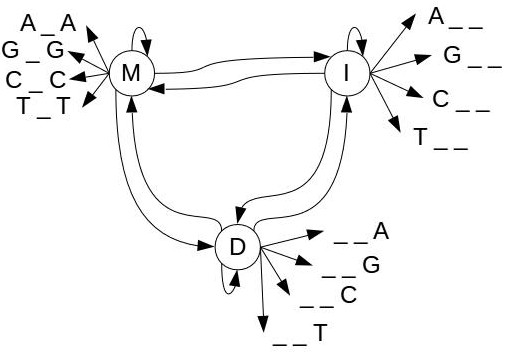
\includegraphics[width=0.7\textwidth]{lectures/160523_2/pix/7.jpg}

M: Match, I: Insertion, D: Deletion\\

Grammatik:
\begin{itemize}
	\item M $\to M_{A\_A} | ... | I | D$
	\item I $\to I_{A\_\_} | ... | D | M$
	\item D $\to D_{\_\_A} | ... | M | I$
\end{itemize}

Beispiel:\\
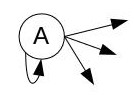
\includegraphics[width=0.1\textwidth]{lectures/160523_2/pix/8.jpg}
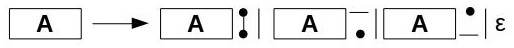
\includegraphics[width=0.7\textwidth]{lectures/160523_2/pix/9.jpg}

\underline{Faltungsgrammatik}\\\\
S $\to (S)S | .S| \varepsilon$\\
Nichtterminale = S, Alphabet = \{(, ), .\}\\

\newpage

Beispiel in Baumdarstellung:\\
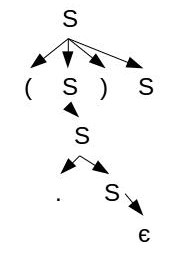
\includegraphics[width=0.2\textwidth]{lectures/160523_2/pix/10.jpg}

weiteres Beispiel: Sankoff, Kombination von zwei Grammatiken (Alignment und Faltung)\\\\
\underline{Alignmentgrammatik}\\\\
S $\to .S | \_S | \varepsilon$\\
G = $(N = \{S\}, \Sigma = \{., \_\}, P=\{S \to .S | \_S | \varepsilon\}, S)$\\
Alignment: $G^2 = G \times G = (N \times N, \Sigma \times \Sigma, P^2, (S,S))$\\
$P^2 = P \times P = 
\left(
    \begin{array}{c}
      S \\
      S
    \end{array}
  \right)
$